\section{Tools}

\subsection{Code editor}

For developing this project, some tools have been used. We will analyze them here and see why they
have been used.

The first tool used has been the code editor. The editor used has been Sublime
Text~\cite{sublime_web}. We were using version 2 until March 2015, where development in version 3
gave life signs and we decided to upgrade the version. There are multiple \acrshort{ide}s such as
PyCharm~\cite{pycharm_web}, Eclipse~\cite{eclipse_web} or other editors such as
Atom~\cite{atom_web}, Lime Text~\cite{lime_web} or Microsoft Visual Studio Code~\cite{ms_code_web}.
There are also other console tools like Vim~\cite{vim_web}, Nano~\cite{nano_web} or
Emacs~\cite{emacs_web}.

Nevertheless, even if I would have preferred to work with an open source editor, the truth is that
currently, the closed sourced ones offer better performance. For instance, Atom tries to be the
open source alternative to Sublime Text, but it starts really slowly and the plug-ins for Sublime
Text can be found for almost every situation. Lime Text might outperform Sublime Text in the future
but currently it is still in an unstable release. Microsoft Visual Studio Code was released later
this year and it did not have any benefit with respect to Sublime Text, so it was worthless changing
the editor at this point.

On the other hand, \acrshort{ide}s are big softwares that from my point of view interfere in the
programming process. In the end, this is about feeling comfortable with the tool, and the velocity
and simplicity offered by editors outperform \acrshort{ide}s greatly. That is why the tool used for
all the programming (except the Arduino script) has been Sublime Text 3 (figure~\ref{fig:sublime}).

\begin{figure}[!htbp]
	\centering
	
\includegraphics[width=0.3\textwidth]{fig/sublime}
	\caption{Sublime Text logo.}
	\label{fig:sublime}
\end{figure}

Nevertheless, since the robot's microcontroller is an Arduino, the Arduino
\acrshort{ide}~\cite{arduino_web} (figure~\ref{fig:arduino}) has been used to program the robot
itself, since it is simple and easy to use for this simple task. For some specific situations such
as small testing changes made in the project's Raspberry Pi or testing server configuration Nano
has been used since it provides a simple console interface easy to use when connecting via
\acrshort{ssh} (\acrlong{ssh}).

\begin{figure}[!htbp]
	\centering
	
\includegraphics[width=0.6\textwidth]{fig/arduino}
	\caption{Arduino Community logo. \emph{Source: Arduino}}
	\label{fig:arduino}
\end{figure}

\subsection{User interface testing}

Since one of the key points of the project has been the user interface and in overall the web client
of the system, this needed to be tested. For this task, two main web browsers have been used:
Mozilla Firefox~\cite{firefox_web} (figure~\ref{subfig:firefox}) and Google Chrome~\cite{chrome_web}
(figure~\ref{subfig:chrome}). Here, it has been found that Google Chrome's developer tools have
helped the development more, thanks to their features and ease of use. We can see a screenshot of
Google Chrome's developer tools in figure~\ref{fig:chrome_dev}.

\begin{figure}[!htbp]
	\centering
	\begin{subfigure}{0.45\textwidth}
		\centering
		
\includegraphics[width=0.5\textwidth]{fig/firefox}
		\caption{Mozilla Firefox logo.}\label{subfig:firefox}
	\end{subfigure}\quad
	\begin{subfigure}{0.45\textwidth}
		\centering
		
\includegraphics[width=0.5\textwidth]{fig/chrome}
		\caption{Google Chrome's logo.}\label{subfig:chrome}
	\end{subfigure}\quad
	\caption{Web browsers used for testing.}
\end{figure}

\begin{figure}[!htbp]
	\centering
	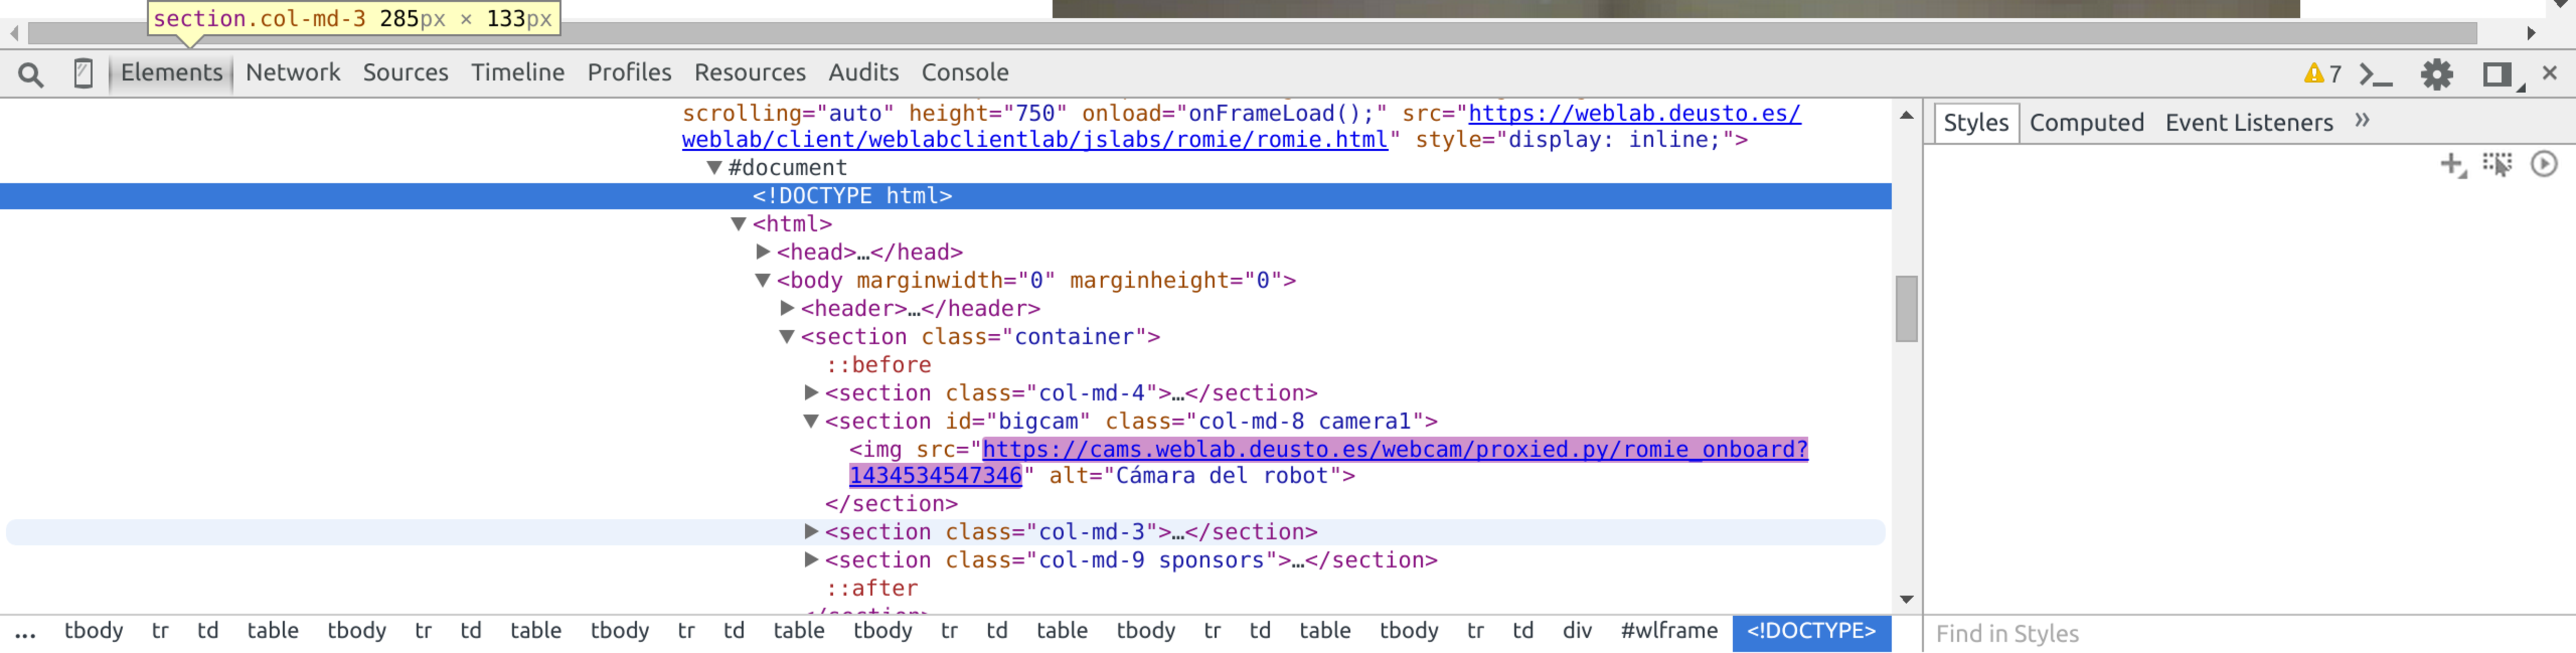
\includegraphics[width=0.95\textwidth]{fig/chrome-dev}
	\caption{Google Chrome's developer tools.}
	\label{fig:chrome_dev}
\end{figure}

\subsection{Operating system and tools}

For the development, the \acrlong{os} used has been Ubuntu \acrshort{gnome}~\cite{ubuntu_gnome_web}
(figure~\ref{subfig:ubuntu_gnome}). This distribution gives all the needed productivity and user
friendliness. The user interface used has been \acrshort{gnome} Shell, and as far as possible, it
has been tried to use only \acrshort{floss} software (\acrlong{floss}).

Moreover, for the server environments two main operating systems have been used: Ubuntu
Server~\cite{ubuntu_web} (figure~\ref{subfig:ubuntu}) and Raspbian~\cite{raspbian_web}, the
Raspberry Pi \acrshort{arm} compatible Debian~\cite{debian_web} distribution
(figure~\ref{subfig:debian}). The first of the two has been used for main WebLab-Deusto servers. It
is used due to its user friendliness, even if being a \acrshort{cli} interface (\acrlong{cli}). The
second one has been used due to its compatibility with the hardware being used for the project, the
Raspberry Pi computer.

\begin{figure}[!htbp]
	\centering
	\begin{subfigure}{0.3\textwidth}
		\centering
		
\includegraphics[width=0.75\textwidth]{fig/ubuntu-gnome}
		\caption{Ubuntu \acrshort{gnome} logo.}\label{subfig:ubuntu_gnome}
	\end{subfigure}\quad
	\begin{subfigure}{0.3\textwidth}
		\centering
		
\includegraphics[width=0.75\textwidth]{fig/ubuntu}
		\caption{Ubuntu logo.}\label{subfig:ubuntu}
	\end{subfigure}\quad
	\begin{subfigure}{0.3\textwidth}
		\centering
		
\includegraphics[width=0.75\textwidth]{fig/debian}
		\caption{Debian logo.}\label{subfig:debian}
	\end{subfigure}\quad
	\caption{Operating systems used in this project.}
\end{figure}

In all cases, the communication between the various servers has been done via \acrshort{ssh}, since
it provides an easy interface with the consoles of the servers.

\subsection{Version control}

For the version control of the project, Git~\cite{git_web} has been used (figure~\ref{subfig:git}).
Git is a distributed version control system created by Linus Torvalds to improve the Linux kernel
development. It allows having repositories distributed without a need of a central repository.
Nevertheless, we have used GitHub~\cite{github_web} for the Git hosting as well as for issue
tracking since GitHub provides with a simple issue management interface, with integrated pull
requests, simple and effective.

\begin{figure}[!htbp]
	\centering
	\begin{subfigure}{0.6\textwidth}
		\centering
		
\includegraphics[width=0.8\textwidth]{fig/git.eps}
		\caption{Git logo.}\label{subfig:git}
	\end{subfigure}\quad
	\begin{subfigure}{0.3\textwidth}
		\centering
		
\includegraphics[width=0.8\textwidth]{fig/github}
		\caption{GitHub's octocat logo.}\label{subfig:github}
	\end{subfigure}\quad
	\caption{Tools and services used for version control.}
\end{figure}

\section{Technology}

In this section we will analyze the technology and tools used for this project.

TODO: Hardware/software: Raspberry, Python, HTML 5, JavaScript, JSON, HTTP, REST, Bluetooth,
